% FERRAMENTAS UTILIZADAS-------------------------------------------------------------------

\chapter{FERRAMENTAS UTILIZADAS}
\label{chap:ferramentas_utilizadas}

Esse capítulo tem por objetivo listar e definir, de forma resumida, todas as ferramentas que foram necessárias para que a versão final do projeto fosse criada. As ferramentas listadas abaixo abordam desde a criação do projeto e hospedagem do seu repositório em uma plataforma \online{} até a documentação do mesmo e apresentação final:

\begin{itemize}
    \item \textbf{Adaptive DSD:} algoritmo de diagnóstico/detecção de falhas em um sistema distribuído. 
    \item \textbf{Bootstrap:} \textit{kit} de ferramentas de código aberto para desenvolvimento com HTML, CSS e JS.
    \item \textbf{CSS:} linguagem que descreve o estilo de um documento HTML.
    \item \textbf{Docker:} ferramenta para facilitar a criação e execução de aplicação utilizando \containers{}.
    \item \textbf{Firebase:} plataforma de desenvolvimento de aplicativos que funciona como \textit{BaaS} (\textit{Backend as a Service}).
    \item \textbf{GIT:} sistema de controle de versões distribuído.
    \item \textbf{GitHub:} plataforma \online{} para armazenar o repositório do projeto.
    \item \textbf{HTML:} linguagem de marcação padrão para páginas da \web{}.
    \item \textbf{Insomnia:} cliente multiplataforma para requisições \textit{GraphQL} e \textit{REST}. 
    \item \textbf{JavaScript:} linguagem de programação.
    \item \textbf{Markdown:} linguagem simples de marcação em texto puro.
    \item \textbf{Mozilla, Chrome:} \textit{browsers}.
    \item \textbf{Oh My Zsh:} \textit{framework} de código aberto para gerenciar a configuração \textit{zsh} do usuário.
    \item \textbf{Postman:} plataforma de colaboração para o desenvolvimento de \textit{API} (Application Programming Interface).
    \item \textbf{PWA:} (\textit{Progressive Web Applications}) é um tipo de \software{} aplicativo fornecido pela \web{}.
    \item \textbf{Python:} linguagem de programação.
    \item \textbf{React:} biblioteca JavaScript para criar interfaces de usuário.
    \item \textbf{Visual Studio Code:} editor de textos utilizado para a codificação da solução.
    \item \textbf{Visual Studio Code (Plugins):} extensões adicionadas ao editor de textos para facilitar o trabalho ou aumentar a produtividade, tais como:
    \begin{itemize}
        \item \textit{LaTex Workshop}
        \item \textit{React-Native/React/Redux snippets for es6/es7}
        \item \textit{Auto Import}
        \item \textit{JavaScript (ES6) code snippets}
        \item \textit{Live Share}
    \end{itemize}
\end{itemize}




% Áreas Envolvidas-------------------------------------------------------------------
\section{Áreas Envolvidas}
\label{sec:areas_envolvidas}

Essa seção irá apresentar todas as disciplinas que foram envolvidas na realização deste trabalho, uma vez que o objetivo da matéria de \textbf{Laboratório de Desenvolvimento} é integrar os conhecimentos já vistos em outras cadeiras do curso e colocá-los em prática em um projeto que solucione ou aborde um problema real do cotidiano. No entanto, ao invés de escrever vários parágrafos que descreveriam cada uma das disciplinas e em qual parte do projeto seus conceitos foram necessários, o grupo optou por criar um diagrama:

\begin{figure}[!htb]
    \centering
    \caption{Diagrama de Relação: Disciplinas x Projeto}
    \frame{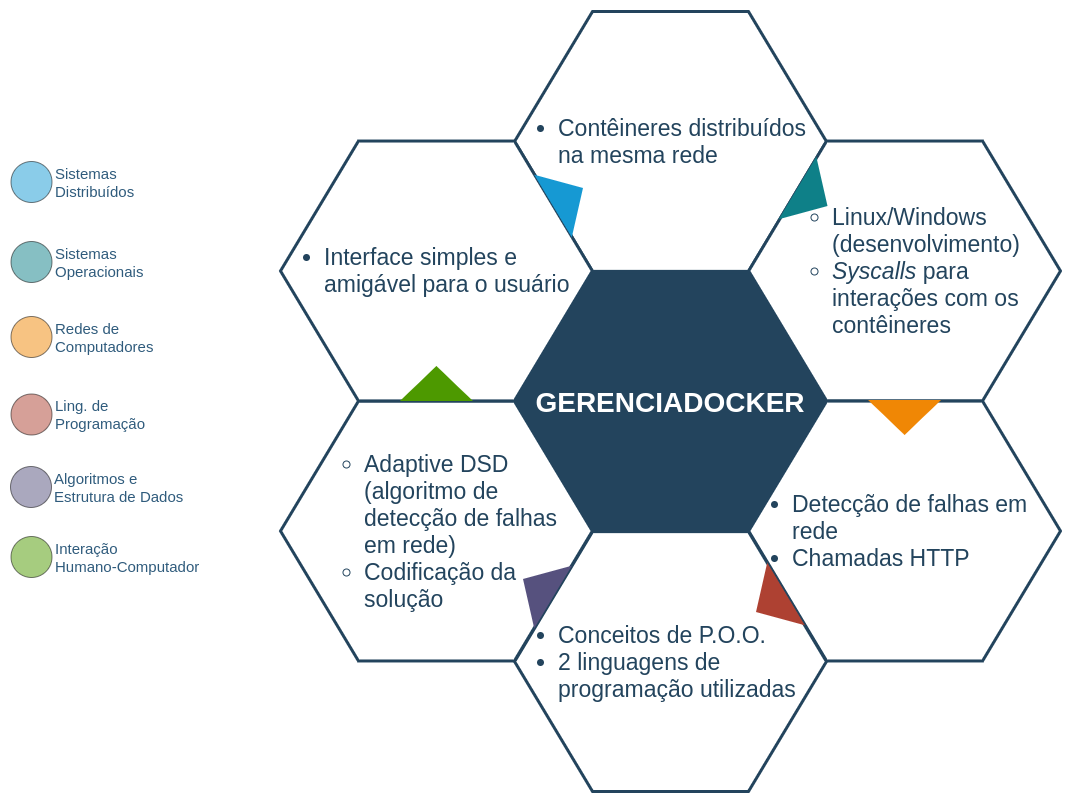
\includegraphics[width=1.0\textwidth]{./content/textuais/imagens/areas_envolvidas.png}}
    \label{fig:areas_envolvidas}
\end{figure}

O objetivo deste diagrama é proporcionar uma visualização mais simples dessa relação \aspas{disciplinas x projeto}, além de facilitar a leitura do documento como um todo. Como é possível ver na figura \ref{fig:areas_envolvidas}, ao centro do diagrama está o projeto e, circundando-o, estão todas as tarefas realizadas durante sua execução. Por fim, para ilustrar à qual disciplina cada tarefa pertence, pode-se notar uma legenda na parte esquerda da figura.